\documentclass[11pt,a4paper]{article}

% --- Single-column, continuous layout ---
\usepackage[margin=1in]{geometry}
\usepackage{parskip}
\usepackage{microtype}

% --- Typography ---
\usepackage[T1]{fontenc}
\usepackage{lmodern}

% --- Graphics, diagrams, code ---
\usepackage{graphicx}
\usepackage{tikz}
\usetikzlibrary{arrows.meta, positioning, shapes.geometric, fit, backgrounds, calc}
\usepackage{listings}
\usepackage{xcolor}
\usepackage{seqsplit}
\usepackage{booktabs}
\usepackage{array}
\usepackage{amsmath}
\usepackage{amssymb}
\usepackage{amsthm}
\newtheorem{theorem}{Theorem}
\usepackage{hyperref}
\hypersetup{colorlinks=true, linkcolor=blue!50!black, urlcolor=blue!50!black, citecolor=blue!50!black, breaklinks=true}
\usepackage{xurl}  % must come after hyperref; enables URL line breaks

% --- Allow long inline paths/URLs to break across lines ---
\sloppy
\emergencystretch=3em

% Helper: a breakable typewriter path (allows linebreaks at / and _)
\newcommand{\bpath}[1]{\texttt{\seqsplit{#1}}}

% --- Listings style for Python ---
\definecolor{codebg}{RGB}{248,248,250}
\definecolor{codecomment}{RGB}{106,135,89}
\definecolor{codekeyword}{RGB}{0,82,156}
\definecolor{codestring}{RGB}{163,21,21}
\definecolor{codenumber}{RGB}{120,120,120}

\lstdefinestyle{pystyle}{
    backgroundcolor=\color{codebg},
    basicstyle=\ttfamily\small,
    commentstyle=\color{codecomment}\itshape,
    keywordstyle=\color{codekeyword}\bfseries,
    stringstyle=\color{codestring},
    numberstyle=\tiny\color{codenumber},
    numbers=left,
    numbersep=8pt,
    showstringspaces=false,
    breaklines=true,
    frame=single,
    rulecolor=\color{black!20},
    framerule=0.4pt,
    aboveskip=10pt,
    belowskip=10pt,
    captionpos=b,
    language=Python,
    tabsize=4,
}
\lstset{style=pystyle}

% --- TikZ shared styles ---
\tikzset{
    agent/.style={
        rectangle, rounded corners=2pt,
        draw=blue!60!black, fill=blue!8,
        minimum width=2.4cm, minimum height=0.9cm,
        font=\small\sffamily, align=center, thick
    },
    director/.style={
        rectangle, rounded corners=2pt,
        draw=red!60!black, fill=red!10,
        minimum width=2.6cm, minimum height=0.9cm,
        font=\small\sffamily\bfseries, align=center, thick
    },
    io/.style={
        ellipse, draw=black!60, fill=gray!10,
        minimum width=2cm, minimum height=0.7cm,
        font=\small\sffamily, align=center
    },
    arrow/.style={-Latex, thick, draw=black!70},
    parallelarrow/.style={-Latex, thick, draw=orange!70!black, dashed},
    group/.style={
        rectangle, rounded corners=4pt,
        draw=black!30, dashed, fill=yellow!4,
        inner sep=8pt
    }
}

\begin{document}

% --- Centered traditional title block ---
\begingroup
\setlength{\parindent}{0pt}
\noindent\rule{\textwidth}{1.6pt}
\vspace{10pt}
\begin{center}
{\LARGE\bfseries AgentRearrange: A General-Purpose Multi-Agent Orchestrator\par}
\end{center}
\vspace{4pt}
\noindent\rule{\textwidth}{0.6pt}
\vspace{14pt}

\begin{center}
{\normalsize Kye Gomez$^{1,*}$,\quad Kuanting Kuo$^{1}$,\quad Aditya Chaudhary$^{1}$,\quad Hugh Nguyen$^{1}$,\quad Swarms Research Team$^{1}$\par}
\vspace{6pt}
{\small $^{1}$Swarms\qquad $^{*}$Project Lead\par}
\vspace{4pt}
{\small Correspondence: \href{mailto:kye@swarms.world}{kye@swarms.world}\par}
\end{center}

\vspace{6pt}
\begin{center}{\large\bfseries Abstract}\end{center}
\vspace{-4pt}

\begin{quote}
\noindent
This report introduces \textbf{AgentRearrange}, a multi-agent orchestration primitive in the Swarms framework that lets engineers express arbitrary mixtures of sequential and concurrent agent execution through a tiny, readable flow grammar. Where dedicated structures such as \texttt{SequentialWorkflow} and \texttt{ConcurrentWorkflow} fix a single topology at construction time, AgentRearrange separates \emph{topology} from \emph{instantiation}: a workflow is a string like \texttt{"researcher -> writer, reviewer -> editor"}, parsed at runtime into an executable schedule. We describe the motivation behind the abstraction, the parsing and scheduling model, the team-awareness mechanism that lets each agent see its upstream and downstream neighbors, and the supporting features for batched, concurrent, asynchronous, and token-streaming execution. We then present architectural diagrams for the canonical patterns AgentRearrange enables (linear pipelines, fan-out/fan-in, diamonds, and human-in-the-loop hops), followed by runnable code examples. The implementation is open-source under Apache-2.0, ships in the \texttt{swarms} package on PyPI, and is available at \href{https://github.com/kyegomez/swarms}{\texttt{github.com/kyegomez/swarms}}.
\end{quote}

\vspace{10pt}
\endgroup

\section{Introduction}

The dominant pattern in multi-agent systems literature is to pick a topology (sequential, concurrent, hierarchical, debate) and bake it into a class. Each topology becomes its own primitive: \texttt{SequentialWorkflow} for pipelines, \texttt{ConcurrentWorkflow} for fan-outs, \texttt{HierarchicalSwarm} for boss-worker delegation, and so on. This design is clean for textbook examples but becomes awkward the moment a real-world workflow needs a \emph{mix} of behaviors, for instance a research agent feeding two parallel writers whose drafts are then merged by an editor.

The Swarms framework introduces \textbf{AgentRearrange}, a structure whose only configuration is a flow string and a list of agents. The flow string is a compact domain-specific language (DSL) with two operators: \texttt{->} denotes sequential dependence ("the right side waits for the left"), and \texttt{,} denotes concurrent execution on the same upstream input. These two operators compose, so workflows like \texttt{"a -> b, c -> d"} ("a runs, then b and c run in parallel, then d aggregates") read almost like ASCII art of the underlying DAG.

The contribution of AgentRearrange is not novel scheduling theory; topological execution of a DAG is decades old. The contribution is \emph{ergonomic}: the abstraction lowers the cognitive cost of describing a workflow to the point where engineers can iterate on topology as quickly as they iterate on prompts. A workflow is no longer a class hierarchy; it is a string. Reordering agents, inserting a parallel review step, or fanning out to multiple model providers is a one-line edit. This matters in practice because most multi-agent systems do not arrive at their final shape on day one; they evolve through experimentation, and the friction of restructuring an orchestration is often the bottleneck.

This report walks through why the abstraction exists, how it is implemented in \bpath{swarms/structs/agent\_rearrange.py},\footnote{\href{https://github.com/kyegomez/swarms/blob/master/swarms/structs/agent_rearrange.py}{\bpath{swarms/structs/agent\_rearrange.py}} on GitHub.} the patterns it enables, and the supporting features (streaming, batched execution, asynchronous integration) that turn the core primitive into a production-ready building block.

\section{Background and Motivation}

Early Swarms users repeatedly hit the same wall. They would prototype a research workflow with \texttt{SequentialWorkflow}, get it working, then realize the middle stage should actually be three agents running in parallel and merging their outputs. The fix required swapping orchestration classes, refactoring the agent list, and re-threading the conversation history. The workflow shape was \emph{baked into the orchestrator type}, so every shape change cost a rewrite.

A second class of users wanted to A/B test workflow topologies. Given five agents, does \texttt{a -> b -> c -> d -> e} produce better outputs than \texttt{a -> (b, c) -> (d, e)}? Or than \texttt{a -> b -> (c, d) -> e}? Answering these questions required maintaining several orchestrator instances, each in a slightly different shape, often with subtle drift in how they handled conversation state.

The third pain point was \emph{readability}. Reading a 30-line orchestrator setup with conditional graph construction tells you very little about what the workflow actually does. By contrast, the string \texttt{"researcher -> analyst, critic -> editor -> publisher"} tells a reader exactly how data flows in fewer characters than a tweet.

AgentRearrange was designed to collapse these three problems into one. The design constraints were:

\begin{itemize}
    \item \textbf{Topology as data, not code.} Flow lives in a string that can be edited, generated, or fed from a config file, not a class hierarchy.
    \item \textbf{Grammar minimal enough to memorize.} Two operators, both ASCII, both readable left-to-right.
    \item \textbf{One conversation, one source of truth.} Every agent reads from and writes to the same \texttt{Conversation} object so context propagates correctly across both sequential and parallel hops.
    \item \textbf{No special-casing.} Every other Swarms structure ultimately reduces to a flow string; if AgentRearrange covers the general case, the dedicated structures become specialized factories on top of it.
    \item \textbf{Production-ready surface.} Sync, async, streaming, batched, and concurrent execution all available without changing the flow.
\end{itemize}

The result is the primitive described in the remainder of this report.

\section{Core Design: The Flow DSL}

The flow string is the heart of AgentRearrange. Its grammar fits on one line:

\begin{verbatim}
    flow      := step ("->" step)*
    step      := agent_name ("," agent_name)*
\end{verbatim}

A \emph{step} is a comma-separated list of agent names; agents in the same step execute concurrently and share the same input. The \texttt{->} operator separates steps; the right-hand step begins only after every agent in the left-hand step has finished. The parser is intentionally trivial: a single \texttt{split("->")} followed by \texttt{split(",")} on each segment, which both keeps the implementation auditable and makes the semantics unambiguous.

Three illustrative examples:

\begin{itemize}
    \item \texttt{"a -> b -> c"}: pure sequential pipeline (semantically equivalent to \texttt{SequentialWorkflow}).
    \item \texttt{"a, b, c"}: pure concurrent fan-out (semantically equivalent to \texttt{ConcurrentWorkflow}), though note that flow validation requires at least one \texttt{->}.
    \item \texttt{"a -> b, c -> d"}: diamond. \texttt{a} feeds both \texttt{b} and \texttt{c} in parallel; both then feed \texttt{d}.
\end{itemize}

The same agent name may appear in multiple steps. \texttt{"writer -> reviewer -> writer"} is a valid flow expressing a revise-then-rewrite loop, and the implementation preserves outputs from each occurrence separately so a repeated agent's runs are not silently overwritten.

\subsection{Validation Semantics}

\texttt{validate\_flow()} runs at the start of every \texttt{run()}. It checks two invariants: (1) the flow contains at least one \texttt{->} (preventing accidentally passing a single agent name and getting silent single-shot execution), and (2) every agent name referenced in the flow has been registered in the \texttt{agents} dict. Failures raise a \texttt{ValueError} with the offending name, surfacing typos immediately rather than letting them silently fall through.

\subsection{Conversation as the Shared Bus}

A subtle but consequential design choice: every agent in an AgentRearrange flow reads its input from a shared \texttt{Conversation} object via \texttt{conversation.get\_str()}, and writes its output back to the same object. This is true for both sequential and concurrent steps. A sequential agent sees everything that came before it; a parallel agent sees the same prefix as its peers and writes alongside them.

The implication is that information propagates monotonically: each agent sees the full accumulated transcript up to the moment its step begins. This makes the system easy to reason about (there is no hidden message routing) and easy to debug (the conversation log is the complete execution trace).

\subsection{Semantics}

The shared-conversation discipline above admits a compact formal statement: information accumulates one layer at a time, and within a layer every agent sees the same input. This is the single property from which the correctness of every pattern below follows.

\begin{theorem}[Monotone Layered Execution]
Let a flow string parse into an ordered sequence of steps $S_1 \to S_2 \to \cdots \to S_n$, where each step $S_k$ is a non-empty set of agents. Let $C_k$ denote the contents of the shared conversation immediately before step $S_k$ begins, with $C_1$ the initial task. Then for every $k \in \{1, \ldots, n\}$:
\begin{enumerate}
    \item every agent $a \in S_k$ reads the same input $C_k$;
    \item $C_{k+1} = C_k \,\cup\, \{\,\mathrm{out}(a) : a \in S_k\,\}$;
    \item consequently $C_k = C_1 \,\cup\, \bigcup_{j<k}\mathrm{out}(S_j)$, so each agent observes the complete output of every earlier step.
\end{enumerate}
\end{theorem}

\begin{proof}
By construction. The parser produces the ordered list $(S_1, \ldots, S_n)$ via \texttt{split("->")}, and \texttt{\_run} iterates it in order. Within a step, every agent is dispatched (sequentially when $|S_k|=1$, or via \texttt{run\_agents\_concurrently} when $|S_k|>1$) from the same snapshot of the conversation, and outputs are appended only after the step completes; the \texttt{Conversation} object is append-only within a run. Properties (1) and (2) are therefore immediate, and (3) follows by induction on $k$.
\end{proof}

The theorem makes the fan-in behavior of the diamond pattern (Figure~\ref{fig:diamond}) a corollary rather than a special case: the downstream agent automatically reads both parallel outputs because they were both appended to $C_k$ before it ran.

\section{Architecture and Implementation}

The class lives in \bpath{swarms/structs/agent\_rearrange.py} and clocks in at roughly 1,300 lines including extensive docstrings. The core execution loop is short; most of the file is supporting machinery for telemetry, serialization, and the streaming variants.

\subsection{Lifecycle}

\begin{enumerate}
    \item \textbf{Construction.} \texttt{\_\_init\_\_} stores the agent list as a \texttt{dict} keyed by \texttt{agent\_name}, instantiates a \texttt{Conversation} with the configured name and time settings, optionally injects a system-level \texttt{rules} message, and runs \texttt{reliability\_check()} which verifies the agent list, flow, \texttt{max\_loops}, and \texttt{output\_type} are non-empty and well-formed.
    \item \textbf{Optional team awareness.} If \texttt{team\_awareness=True}, the constructor injects a system message describing the full flow structure (step numbering, predecessors, successors), so agents begin execution already knowing where they sit in the pipeline.
    \item \textbf{Execution.} \texttt{run()} delegates to the private \texttt{\_run()}, wrapping it in telemetry logging and a try/except that routes failures through \texttt{\_catch\_error()} for graceful logging and autosave.
    \item \textbf{Step iteration.} \texttt{\_run} splits the flow on \texttt{->} into a list of steps, then walks the list. For each step it splits on \texttt{,}: a single-name step dispatches to \texttt{\_run\_sequential\_workflow}; a multi-name step dispatches to \texttt{\_run\_concurrent\_workflow}.
    \item \textbf{Concurrent dispatch.} The concurrent helper resolves agent names to objects, calls \texttt{run\_agents\_concurrently} (the framework's parallel runner), and writes each output back to the shared conversation in deterministic order.
    \item \textbf{Output formatting.} After all steps complete (and possibly after multiple loops, if \texttt{max\_loops > 1}), \texttt{history\_output\_formatter} converts the conversation to the configured \texttt{output\_type} (\texttt{"all"}, \texttt{"final"}, \texttt{"list"}, or \texttt{"dict"}).
\end{enumerate}

\subsection{Sequential Awareness for Repeated Agents}

A nuance worth highlighting: when the same agent appears in multiple steps (e.g.\ \texttt{"writer -> reviewer -> writer"}), naive position-by-name lookup would always return the first occurrence, leaving the second invocation thinking it sits at step 0. The implementation threads an explicit \texttt{task\_idx} through \texttt{\_get\_sequential\_awareness}, so each invocation gets correctly contextualized awareness (e.g.\ "Agent ahead: reviewer" on the second \texttt{writer} call). The response dict similarly uses indexed keys (\texttt{Writer\_0}, \texttt{Writer\_2}) to preserve outputs from each occurrence.

\subsection{Diagram: Internal Control Flow}

Figure \ref{fig:internal} shows the internal control flow of a single \texttt{run()} call.

\begin{figure}[h]
\centering
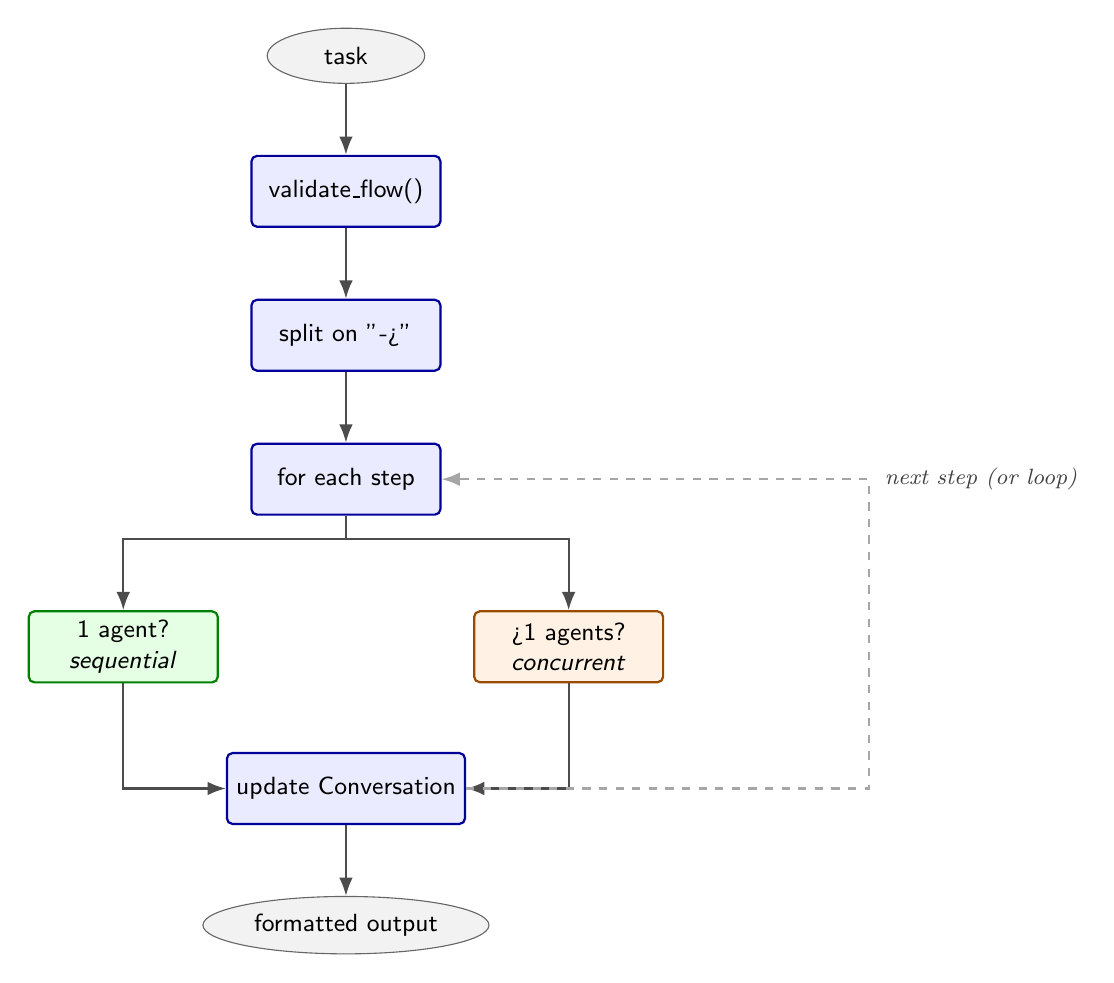
\begin{tikzpicture}[node distance=9mm and 18mm]
    \node[io] (in) {task};
    \node[agent, below=of in] (val) {validate\_flow()};
    \node[agent, below=of val] (split) {split on "->"};
    \node[agent, below=of split] (loop) {for each step};
    \node[agent, below left=12mm and 4mm of loop, fill=green!10, draw=green!50!black] (seq) {1 agent?\\\textit{sequential}};
    \node[agent, below right=12mm and 4mm of loop, fill=orange!10, draw=orange!60!black] (par) {>1 agents?\\\textit{concurrent}};
    \node[agent, below=30mm of loop] (conv) {update Conversation};
    \node[io, below=of conv] (out) {formatted output};

    \draw[arrow] (in) -- (val);
    \draw[arrow] (val) -- (split);
    \draw[arrow] (split) -- (loop);
    \draw[arrow] (loop.south) -- ++(0,-3mm) -| (seq.north);
    \draw[arrow] (loop.south) -- ++(0,-3mm) -| (par.north);
    \draw[arrow] (seq) |- (conv);
    \draw[arrow] (par) |- (conv);

    % Loopback routed far to the right so it doesn't overlap the concurrent node
    \coordinate (rightlane) at ($(par.east) + (2.6,0)$);
    \draw[arrow, dashed, draw=gray!70]
        (conv.east) -| (rightlane)
        |- node[midway, right=2pt, font=\footnotesize\itshape, text=gray!50!black] {next step (or loop)}
        (loop.east);

    \draw[arrow] (conv) -- (out);
\end{tikzpicture}
\caption{Internal control flow of \texttt{AgentRearrange.\_run()}.}
\label{fig:internal}
\end{figure}

\section{Architectural Patterns}

The expressive power of AgentRearrange comes from the patterns it makes trivial to write. Four canonical patterns are shown in figures \ref{fig:sequential}--\ref{fig:hitl}.

\subsection{Linear Pipeline}

\texttt{flow = "researcher -> analyst -> writer -> editor"}

\begin{figure}[h]
\centering
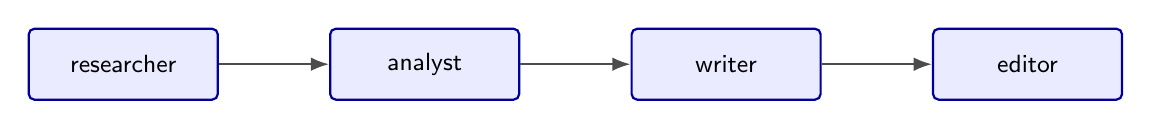
\begin{tikzpicture}[node distance=14mm and 14mm]
    \node[agent] (r) {researcher};
    \node[agent, right=of r] (a) {analyst};
    \node[agent, right=of a] (w) {writer};
    \node[agent, right=of w] (e) {editor};
    \draw[arrow] (r) -- (a);
    \draw[arrow] (a) -- (w);
    \draw[arrow] (w) -- (e);
\end{tikzpicture}
\caption{Linear sequential pipeline.}
\label{fig:sequential}
\end{figure}

\subsection{Fan-out, Fan-in}

\texttt{flow = "ingest -> gpt, claude, gemini -> synthesizer"}

A single source feeds multiple downstream agents in parallel; their outputs converge into a synthesis step. Useful for multi-model ensembling.

\begin{figure}[h]
\centering
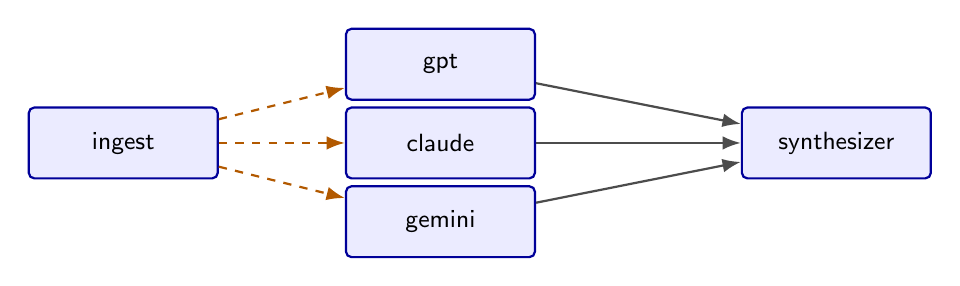
\begin{tikzpicture}[node distance=12mm and 16mm]
    \node[agent] (i) {ingest};
    \node[agent, right=of i, yshift=10mm] (g) {gpt};
    \node[agent, right=of i] (c) {claude};
    \node[agent, right=of i, yshift=-10mm] (gm) {gemini};
    \node[agent, right=of c, xshift=10mm] (s) {synthesizer};

    \draw[parallelarrow] (i) -- (g);
    \draw[parallelarrow] (i) -- (c);
    \draw[parallelarrow] (i) -- (gm);
    \draw[arrow] (g) -- (s);
    \draw[arrow] (c) -- (s);
    \draw[arrow] (gm) -- (s);
\end{tikzpicture}
\caption{Fan-out / fan-in with multi-model ensembling.}
\label{fig:fanout}
\end{figure}

\subsection{Diamond}

\texttt{flow = "planner -> coder, reviewer -> tester"}

The classic diamond shape: one upstream agent, two concurrent middle agents, one downstream aggregator. AgentRearrange handles the join automatically because the shared conversation accumulates both middle outputs before \texttt{tester} reads it.

\begin{figure}[h]
\centering
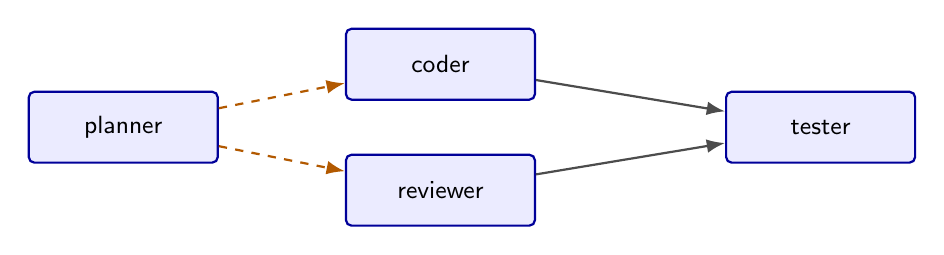
\begin{tikzpicture}[node distance=12mm and 16mm]
    \node[agent] (p) {planner};
    \node[agent, right=of p, yshift=8mm] (c) {coder};
    \node[agent, right=of p, yshift=-8mm] (r) {reviewer};
    \node[agent, right=of c, xshift=8mm, yshift=-8mm] (t) {tester};

    \draw[parallelarrow] (p) -- (c);
    \draw[parallelarrow] (p) -- (r);
    \draw[arrow] (c) -- (t);
    \draw[arrow] (r) -- (t);
\end{tikzpicture}
\caption{Diamond pattern.}
\label{fig:diamond}
\end{figure}

\subsection{Human-in-the-Loop Hop}

\texttt{flow = "drafter -> H -> finisher"} (with \texttt{human\_in\_the\_loop=True})

The \texttt{H} marker designates a human step. The \texttt{custom\_human\_in\_the\_loop} callback receives the upstream output and returns the human's feedback, which is then handed to the downstream agent.

\begin{figure}[h]
\centering
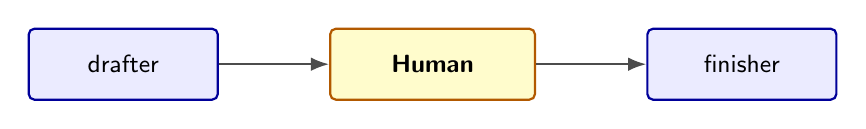
\begin{tikzpicture}[node distance=12mm and 14mm]
    \node[agent] (d) {drafter};
    \node[director, right=of d, fill=yellow!20, draw=orange!70!black] (h) {Human};
    \node[agent, right=of h] (f) {finisher};
    \draw[arrow] (d) -- (h);
    \draw[arrow] (h) -- (f);
\end{tikzpicture}
\caption{Human-in-the-loop hop.}
\label{fig:hitl}
\end{figure}

\subsection{Compound Pattern}

Real workloads combine these. Figure \ref{fig:compound} shows a research pipeline where ingestion feeds two parallel analysts, both feed a writer, the writer is reviewed in parallel by an editor and a fact-checker, and a publisher closes the workflow.

\texttt{flow = "ingest -> analyst\_a, analyst\_b -> writer -> editor, fact\_checker -> publisher"}

\begin{figure}[h]
\centering
\resizebox{\textwidth}{!}{%
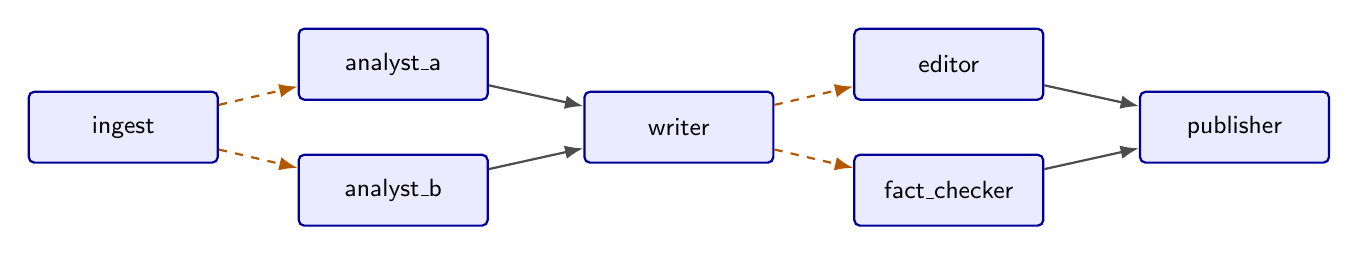
\begin{tikzpicture}[node distance=8mm and 10mm]
    \node[agent] (i) {ingest};
    \node[agent, right=of i, yshift=8mm] (aa) {analyst\_a};
    \node[agent, right=of i, yshift=-8mm] (ab) {analyst\_b};
    \node[agent, right=of aa, xshift=2mm, yshift=-8mm] (w) {writer};
    \node[agent, right=of w, yshift=8mm] (ed) {editor};
    \node[agent, right=of w, yshift=-8mm] (fc) {fact\_checker};
    \node[agent, right=of ed, xshift=2mm, yshift=-8mm] (p) {publisher};

    \draw[parallelarrow] (i) -- (aa);
    \draw[parallelarrow] (i) -- (ab);
    \draw[arrow] (aa) -- (w);
    \draw[arrow] (ab) -- (w);
    \draw[parallelarrow] (w) -- (ed);
    \draw[parallelarrow] (w) -- (fc);
    \draw[arrow] (ed) -- (p);
    \draw[arrow] (fc) -- (p);
\end{tikzpicture}%
}
\caption{Compound pattern combining fan-in, fan-out, and final aggregation.}
\label{fig:compound}
\end{figure}

\section{Code Examples}

\subsection{Minimal Sequential}

\begin{lstlisting}[caption={Minimal sequential pipeline.},label={lst:seq}]
from swarms import Agent, AgentRearrange

researcher = Agent(agent_name="researcher", model_name="gpt-4.1", max_loops=1)
writer     = Agent(agent_name="writer",     model_name="gpt-4.1", max_loops=1)
editor     = Agent(agent_name="editor",     model_name="gpt-4.1", max_loops=1)

system = AgentRearrange(
    agents=[researcher, writer, editor],
    flow="researcher -> writer -> editor",
    max_loops=1,
)
result = system.run("Write an article on the history of transformer architectures.")
\end{lstlisting}

\subsection{Diamond Workflow}

\begin{lstlisting}[caption={Diamond: one upstream, two concurrent middles, one downstream.},label={lst:diamond}]
from swarms import Agent, AgentRearrange

planner  = Agent(agent_name="planner",  model_name="gpt-4.1", max_loops=1)
coder    = Agent(agent_name="coder",    model_name="gpt-4.1", max_loops=1)
reviewer = Agent(agent_name="reviewer", model_name="gpt-4.1", max_loops=1)
tester   = Agent(agent_name="tester",   model_name="gpt-4.1", max_loops=1)

pipeline = AgentRearrange(
    agents=[planner, coder, reviewer, tester],
    flow="planner -> coder, reviewer -> tester",
    max_loops=1,
    team_awareness=True,  # tell each agent its neighbors
)
result = pipeline.run("Build a Python function that validates email addresses.")
\end{lstlisting}

\subsection{Multi-Model Ensemble Fan-Out / Fan-In}

\begin{lstlisting}[caption={Three model providers in parallel, one synthesizer.},label={lst:moa}]
from swarms import Agent, AgentRearrange

ingest = Agent(agent_name="ingest", model_name="gpt-4.1", max_loops=1)

gpt    = Agent(agent_name="gpt",    model_name="gpt-4.1",          max_loops=1)
claude = Agent(agent_name="claude", model_name="claude-sonnet-4-6", max_loops=1)
gemini = Agent(agent_name="gemini", model_name="gemini/gemini-2.5-pro", max_loops=1)

synth  = Agent(
    agent_name="synthesizer",
    model_name="gpt-4.1",
    system_prompt="Combine the three expert responses into one coherent answer.",
    max_loops=1,
)

ensemble = AgentRearrange(
    agents=[ingest, gpt, claude, gemini, synth],
    flow="ingest -> gpt, claude, gemini -> synthesizer",
    max_loops=1,
)
print(ensemble("What is the most underrated breakthrough in deep learning since 2020?"))
\end{lstlisting}

\subsection{Repeated Agent (Revise Loop)}

\begin{lstlisting}[caption={The same writer is invoked twice with a review in between.},label={lst:revise}]
from swarms import Agent, AgentRearrange

writer   = Agent(agent_name="writer",   model_name="gpt-4.1", max_loops=1)
reviewer = Agent(agent_name="reviewer", model_name="gpt-4.1", max_loops=1)

revise = AgentRearrange(
    agents=[writer, reviewer],
    flow="writer -> reviewer -> writer",  # same agent, two invocations
    max_loops=1,
    team_awareness=True,
)
result = revise.run("Draft, critique, then revise a short essay on Hannah Arendt.")
\end{lstlisting}

\subsection{Batched and Concurrent Multi-Task Execution}

\begin{lstlisting}[caption={Running the same flow over many independent tasks.},label={lst:batch}]
from swarms import Agent, AgentRearrange

a = Agent(agent_name="extract",   model_name="gpt-5.4-mini", max_loops=1)
b = Agent(agent_name="transform", model_name="gpt-5.4-mini", max_loops=1)
c = Agent(agent_name="load",      model_name="gpt-5.4-mini", max_loops=1)

etl = AgentRearrange(
    agents=[a, b, c],
    flow="extract -> transform -> load",
)

tasks = [f"Process document {i}.pdf" for i in range(50)]

# Batched: deep-copies isolate state per task, batch_size at a time.
batch_results = etl.batch_run(tasks=tasks, batch_size=10)

# Concurrent: ThreadPoolExecutor across all tasks at once.
parallel_results = etl.concurrent_run(tasks=tasks, max_workers=8)
\end{lstlisting}

\subsection{Async and Streaming}

\begin{lstlisting}[caption={Async execution and token-level streaming.},label={lst:stream}]
import asyncio
from swarms import Agent, AgentRearrange

a = Agent(agent_name="a", model_name="gpt-4.1", max_loops=1)
b = Agent(agent_name="b", model_name="gpt-4.1", max_loops=1)
c = Agent(agent_name="c", model_name="gpt-4.1", max_loops=1)

ar = AgentRearrange(agents=[a, b, c], flow="a -> b, c")

async def main():
    # Awaitable result
    result = await ar.run_async("Explain modular arithmetic with examples.")
    print(result)

    # Token-by-token stream; for parallel steps, tokens from b and c interleave.
    async for agent_name, token in ar.arun_stream("Explain it again, briefly."):
        print(f"[{agent_name}] {token}", end="", flush=True)

asyncio.run(main())
\end{lstlisting}

\section{Advanced Features}

\subsection{Team Awareness}

Setting \texttt{team\_awareness=True} injects two pieces of context. At construction time, the system message receives a description of the full flow structure: each step numbered, with its predecessors and successors listed. At execution time, before each sequential agent runs, an additional system message is appended naming the agents directly ahead and behind in the sequence. The intent is to give the agent enough situational awareness to write outputs that the next agent can consume cleanly, without having to encode "you are step 3 of 5" into every prompt by hand.

\subsection{Streaming with Fair Interleaving}

The streaming variants (\texttt{arun\_stream}, \texttt{run\_stream}) yield tokens as they arrive. Sequential steps stream tokens from one agent at a time; parallel steps interleave tokens from concurrent agents via an asyncio queue. A deliberate \texttt{await asyncio.sleep(0)} sits between yields in the parallel path; without it the consumer would drain one producer's burst before the scheduler hopped to the next, producing a clumpy \texttt{AAAA...BBBB} pattern instead of the fairer \texttt{ABABAB} weave users expect from a parallel stream. The \texttt{with\_events=True} flag swaps the tuple yield for structured event dicts (\texttt{agent\_start}, \texttt{token}, \texttt{agent\_end}), which is the form most useful for wiring into a server-sent-events handler.

\subsection{Batched vs.\ Concurrent Multi-Task Execution}

\texttt{batch\_run} processes tasks in chunks of \texttt{batch\_size}, deep-copying the entire orchestrator per task so conversation state is fully isolated. Each chunk runs on a thread pool sized by CPU count. This is the right choice when conversation history must not bleed across tasks; for example, when each task is an independent customer query.

\texttt{concurrent\_run}, by contrast, fires all tasks into a single \texttt{ThreadPoolExecutor} bounded by \texttt{max\_workers}, with the same orchestrator instance reused. This is faster but assumes the workload tolerates a shared underlying state. For pure I/O-bound flows where every agent calls out to an LLM API, this is usually fine.

\subsection{The \texttt{rearrange} Convenience Function}

For one-shot use, the module exports a \texttt{rearrange()} function that constructs an \texttt{AgentRearrange}, runs the given task, and returns the result in a single call. It is purely a thin convenience wrapper but reduces a five-line construct to a one-liner for ad-hoc scripts and notebooks.

\section{Comparison with Other Swarms Structures}

AgentRearrange is the most expressive orchestrator in Swarms but not always the right choice. Table \ref{tab:compare} positions it against its siblings.

\begin{table}[h]
\centering
\small
\begin{tabular}{p{3.4cm} p{3.4cm} p{7.5cm}}
\hline
\textbf{Structure} & \textbf{Topology} & \textbf{When to prefer it} \\
\hline
\texttt{SequentialWorkflow} & Linear pipeline & Pure A→B→C; reads marginally cleaner than \texttt{AgentRearrange} for that case. \\
\texttt{ConcurrentWorkflow} & Pure fan-out & Same task to N agents, results collected; no downstream join. \\
\texttt{AgentRearrange} & \textbf{Arbitrary mix} & \textbf{Any time the topology is more than a straight line or a flat fan-out.} \\
\texttt{GraphWorkflow} & Full DAG & When you need per-node callbacks, explicit node IDs, programmatic graph construction, or non-string-expressible dependencies. \\
\texttt{HierarchicalSwarm} & Director + workers & Director must decide \emph{which} workers to invoke per task at runtime, not at flow-definition time. \\
\hline
\end{tabular}
\caption{Choosing among Swarms orchestration structures.}
\label{tab:compare}
\end{table}

The line we draw most often is between \texttt{AgentRearrange} and \texttt{GraphWorkflow}. The flow DSL covers the 80\% case: workflows where the dependency structure can be expressed as a sequence of comma-separated parallel groups. The 20\% it does not cover (arbitrary cross-step edges such as a step-3 agent feeding both a step-2 and a step-5 agent, per-node callbacks, or dependency graphs built programmatically from data) is where \texttt{GraphWorkflow} earns its weight.

\section{Production Considerations}

A few practical notes from running AgentRearrange in production.

\textbf{Agent names must be unique.} The agent list is stored as a dict keyed by \texttt{agent\_name}; duplicates silently overwrite earlier entries. The flow string references agents by name, so a duplicate effectively merges two configurations. Unique, descriptive names are the cheapest reliability investment.

\textbf{Set explicit \texttt{max\_loops}.} The orchestrator's \texttt{max\_loops} re-runs the entire flow that many times, with the conversation continuing to accumulate across loops. This is rarely what users want for a single-shot workflow; leave it at the default 1 unless you have a specific iterative refinement pattern in mind.

\textbf{Watch context length on long flows.} Because every agent reads the full conversation, the input to the last agent in a long flow can be very large. For flows of more than 5--6 steps, enable \texttt{context\_compression=True} on the participating agents so they auto-summarize when nearing the limit.

\textbf{Validate flows in CI.} Because flows are strings, typos slip through. A trivial unit test that instantiates each orchestrator with its production flow and an empty task will surface every "Agent 'X' is not registered" error at test time rather than at 3 a.m.

\textbf{Use \texttt{rules}, not prompt-engineering each agent.} The \texttt{rules} parameter prepends a system message visible to every agent in the flow. For invariants that apply to the entire workflow ("output JSON only", "never reveal internal tokens"), this is far cleaner than appending the same paragraph to each agent's system prompt.

\section{Conclusion and Future Work}

AgentRearrange shows that the right abstraction can collapse what would otherwise be a family of orchestrator classes into a single primitive parameterized by a string. The flow DSL is small enough to memorize, expressive enough to capture the workflows that real systems need, and ergonomic enough that engineers iterate on orchestration topology with the same low friction they apply to prompts. The implementation deliberately delegates parallel execution to existing Swarms machinery (\texttt{run\_agents\_concurrently}), keeps the shared \texttt{Conversation} as the single source of truth, and exposes sync, async, streaming, batched, and concurrent surfaces without changing the underlying flow.

Several directions remain open. First, the current DSL is linear in steps; expressing fully general DAGs with cross-step edges still requires \texttt{GraphWorkflow}. A natural extension is named ports (e.g.\ \texttt{"a -> b -> c, a:tail -> c"}) that let a downstream step pull from any earlier step by name rather than only the immediately preceding one. Second, conditional flows ("if the reviewer flags an issue, loop back to writer; otherwise advance to publisher") currently require leaving the DSL behind for Python control flow; a minimal conditional operator would absorb this back into the string. Third, the team-awareness payload could be cached and templated rather than reconstructed per step, removing a small but real source of token overhead on long flows.

The framework is open-source under the Apache-2.0 license. The source for AgentRearrange lives at \href{https://github.com/kyegomez/swarms/blob/master/swarms/structs/agent_rearrange.py}{\bpath{swarms/structs/agent\_rearrange.py}} in the main \href{https://github.com/kyegomez/swarms}{Swarms repository}. Issues, feature requests, and pull requests are welcome.

\section*{Code and Resources}

\begin{center}
\renewcommand{\arraystretch}{1.25}
\begin{tabular}{@{}l@{\hspace{2em}}p{0.62\textwidth}@{}}
\toprule
\textbf{Resource} & \textbf{Location} \\
\midrule
Source repository      & \href{https://github.com/kyegomez/swarms}{github.com/kyegomez/swarms} \\
AgentRearrange source  & \href{https://github.com/kyegomez/swarms/blob/master/swarms/structs/agent_rearrange.py}{\bpath{swarms/structs/agent\_rearrange.py}} \\
Documentation          & \href{https://docs.swarms.world}{docs.swarms.world} \\
PyPI package           & \href{https://pypi.org/project/swarms/}{pypi.org/project/swarms} \\
Marketplace            & \href{https://swarms.world}{swarms.world} \\
Community (Discord)    & \href{https://discord.gg/EamjgSaEQf}{discord.gg/EamjgSaEQf} \\
Twitter / X            & \href{https://twitter.com/swarms_corp/}{@swarms\_corp} \\
License                & Apache-2.0 \\
Version                & Swarms 12.0.0 \\
Contact                & \href{mailto:kye@swarms.world}{kye@swarms.world} \\
\bottomrule
\end{tabular}
\end{center}

\begin{thebibliography}{99}

\bibitem{autogen}
Wu, Q., Bansal, G., Zhang, J., Wu, Y., Zhang, S., Zhu, E., Li, B., Jiang, L., Zhang, X., \& Wang, C.
\newblock {AutoGen: Enabling Next-Gen LLM Applications via Multi-Agent Conversation}.
\newblock \textit{arXiv preprint arXiv:2308.08155}, 2023.

\bibitem{metagpt}
Hong, S., Zheng, X., Chen, J., Cheng, Y., Wang, J., Zhang, C., Wang, Z., Yau, S.K.S., Lin, Z., Zhou, L., Ran, C., Xiao, L., Wu, C., \& Schmidhuber, J.
\newblock {MetaGPT: Meta Programming for a Multi-Agent Collaborative Framework}.
\newblock In \textit{International Conference on Learning Representations (ICLR)}, 2024.

\bibitem{genagents}
Park, J.~S., O'Brien, J.~C., Cai, C.~J., Morris, M.~R., Liang, P., \& Bernstein, M.~S.
\newblock {Generative Agents: Interactive Simulacra of Human Behavior}.
\newblock In \textit{Proceedings of the 36th Annual ACM Symposium on User Interface Software and Technology (UIST)}, 2023.

\bibitem{react}
Yao, S., Zhao, J., Yu, D., Du, N., Shafran, I., Narasimhan, K., \& Cao, Y.
\newblock {ReAct: Synergizing Reasoning and Acting in Language Models}.
\newblock In \textit{International Conference on Learning Representations (ICLR)}, 2023.

\bibitem{reflexion}
Shinn, N., Cassano, F., Gopinath, A., Narasimhan, K., \& Yao, S.
\newblock {Reflexion: Language Agents with Verbal Reinforcement Learning}.
\newblock In \textit{Advances in Neural Information Processing Systems (NeurIPS)}, 2023.

\bibitem{toolformer}
Schick, T., Dwivedi-Yu, J., Dess\`i, R., Raileanu, R., Lomeli, M., Zettlemoyer, L., Cancedda, N., \& Scialom, T.
\newblock {Toolformer: Language Models Can Teach Themselves to Use Tools}.
\newblock In \textit{Advances in Neural Information Processing Systems (NeurIPS)}, 2023.

\bibitem{moa}
Wang, J., Wang, J., Athiwaratkun, B., Zhang, C., \& Zou, J.
\newblock {Mixture-of-Agents Enhances Large Language Model Capabilities}.
\newblock \textit{arXiv preprint arXiv:2406.04692}, 2024.

\bibitem{tot}
Yao, S., Yu, D., Zhao, J., Shafran, I., Griffiths, T.~L., Cao, Y., \& Narasimhan, K.
\newblock {Tree of Thoughts: Deliberate Problem Solving with Large Language Models}.
\newblock In \textit{Advances in Neural Information Processing Systems (NeurIPS)}, 2023.

\bibitem{chainofthought}
Wei, J., Wang, X., Schuurmans, D., Bosma, M., Ichter, B., Xia, F., Chi, E., Le, Q., \& Zhou, D.
\newblock {Chain-of-Thought Prompting Elicits Reasoning in Large Language Models}.
\newblock In \textit{Advances in Neural Information Processing Systems (NeurIPS)}, 2022.

\bibitem{autogpt}
Significant Gravitas.
\newblock {AutoGPT: An Autonomous GPT-4 Experiment}.
\newblock GitHub repository, 2023.
\newblock \url{https://github.com/Significant-Gravitas/AutoGPT}.

\bibitem{langgraph}
LangChain, Inc.
\newblock {LangGraph: Building Stateful, Multi-Actor Applications with LLMs}.
\newblock GitHub repository, 2024.
\newblock \url{https://github.com/langchain-ai/langgraph}.

\bibitem{crewai}
crewAI Inc.
\newblock {CrewAI: Framework for Orchestrating Role-Playing, Autonomous AI Agents}.
\newblock GitHub repository, 2024.
\newblock \url{https://github.com/crewAIInc/crewAI}.

\bibitem{litellm}
BerriAI.
\newblock {LiteLLM: Call All LLM APIs Using the OpenAI Format}.
\newblock GitHub repository, 2024.
\newblock \url{https://github.com/BerriAI/litellm}.

\bibitem{mcp}
Anthropic.
\newblock {Introducing the Model Context Protocol}.
\newblock 2024.
\newblock \url{https://www.anthropic.com/news/model-context-protocol}.

\bibitem{gpt4}
OpenAI.
\newblock {GPT-4 Technical Report}.
\newblock \textit{arXiv preprint arXiv:2303.08774}, 2023.

\bibitem{claude}
Anthropic.
\newblock {The Claude 3 Model Family: Opus, Sonnet, Haiku}.
\newblock Technical report, Anthropic, 2024.

\bibitem{airflow}
Apache Software Foundation.
\newblock {Apache Airflow: A Platform to Programmatically Author, Schedule, and Monitor Workflows}.
\newblock 2014--present.
\newblock \url{https://airflow.apache.org}.

\bibitem{swarms}
Gomez, K. and the Swarms Research Department.
\newblock {Swarms: The Enterprise-Grade Production-Ready Multi-Agent Orchestration Framework}.
\newblock GitHub repository, version 12.0.0, 2024--2026.
\newblock \url{https://github.com/kyegomez/swarms}.

\end{thebibliography}

\end{document}
